The D language is a language inspired by the AWK programming language
\cite{Aho:1987:APL:29361} and the C programming language
\cite{DTrace2004}\cite{Kernighan:1988}. In this chapter, we give a
formal definition of the D programming language that is a part of
OpenDTrace, as well as elaborate on its properties in multithreaded
environments.

\section{Example Script}
\label{sec:example-script}

Before describing the full grammar in detail we present a brief,
example, D script, called a \emph{one liner}.  D one liners are the
most frequently used D scripts because they are an easy way to start
tracing a system without writing a file full of D code.


\begin{figure}
  \centering
  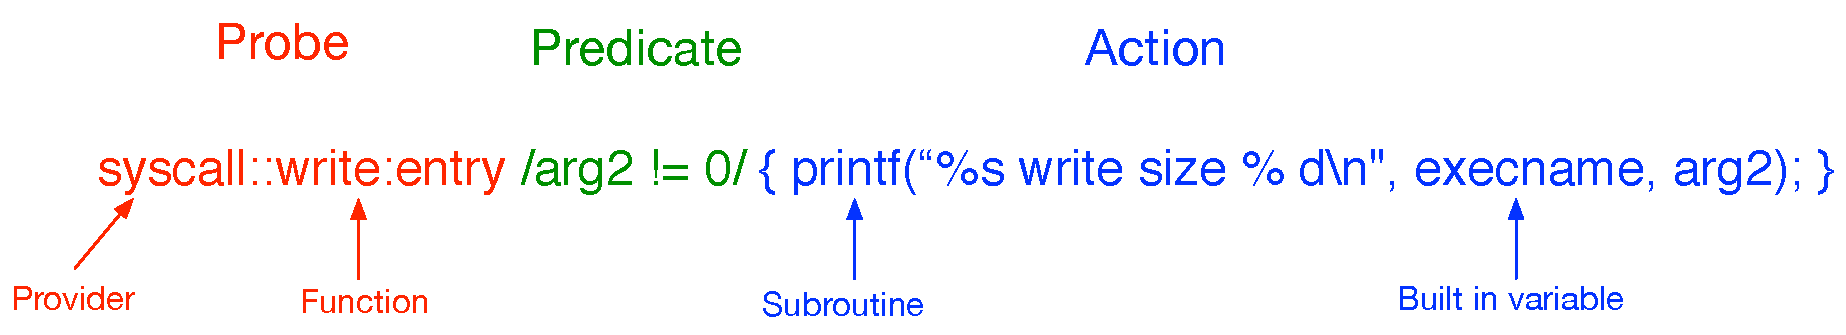
\includegraphics[width=0.8\linewidth]{oneliner.pdf}
  \caption{D One Liner}
  \label{fig:d-one-liner}
\end{figure}

D scripts are a collection of one or more probe points with optional
actions and filtering predicates.  Figure~\ref{fig:d-one-liner} shows
a simple, but descriptive, D script.  The script prints out the size
of the data that a program attempts to write using the
\texttt{write(2)} system call as well as name of the program that made
the write call.  Starting from the left hand side of
Figure~\ref{fig:d-one-liner} we see the probe point in red.  The probe
point includes the provider name, \texttt{syscall} as well as the
function, \texttt{write}, and the fact that we want to look at the
\texttt{entry} into the system call.  Moving to the far right of
Figure~\ref{fig:d-one-liner} we see the action that will be taken
whenever the probe point fires.  Actions are written in the D language
which is an interpreted subset of the C language and so this script
should be familiar to most C or C++ programmers.  D has a large set of
built-in subroutines, described in Chapter~\ref{chap:opendtrace-subroutines},
which includes familiar functions such as \texttt{printf()}.  Each
probe point can have up to six (6) arguments, numbered from arg0 to
arg5, and in this example we are interested in arg2, which is the
\texttt{nbytes} argument to the write system call.  We want to know
which program made the call to \texttt{write} and so we also print the
\texttt{execname} which a D built in variable that contains the name
of the program that caused the probe to fire.

Coming back to the middle of Figure~\ref{fig:d-one-liner} we see text
marked in green, which is a predicate.  Predicates are used to filter
when probes fire allowing the script writer to reduce the amount of
data collected during tracing.  A system call such as \texttt{write}
is called frequently on a busy system and without a predicate the
script will collect quite a bit of data, much of which may not be
relevant to the issue that we are trying to investigate.  The
predicate in Figure~\ref{fig:d-one-liner} allows the probe to fire if,
and only if, the call to \texttt{write} is not equal to zero (0).
More complex boolean expressions are possible within predicates but we
want to have a simple example.

With this example in mind we now turn to the formal grammar for the D
language.

\section{Language grammar}
\label{sec:grammar}

\setlength{\grammarparsep}{5pt plus 1pt minus 1pt} % increase separation between rules
\setlength{\grammarindent}{12em} % increase separation between LHS/RHS

%
\begingroup\makeatletter%
\ifx\bnfdef\undefined%
\gdef\bnfdef{%
  {{$::=$}}%
  }%
\fi%
\ifx\bnfor\undefined%
\gdef\bnfor{%
  {{$\,|\,$}}%
  }%
\fi%
\ifx\bnfopt\undefined%
\gdef\bnfopt#1{%
  {{$\lbrack$ #1 $\rbrack$}}%
  }%
\fi%
\ifx\bnflist\undefined%
\gdef\bnflist#1{%
  {{$\lbrace$ #1 $\rbrace$}}%
  }%
\fi%
\ifx\bnfgroup\undefined%
\gdef\bnfgroup#1{%
  {{$($ #1 $)$}}%
  }%
\fi%
\ifx\bnftoken\undefined%
\gdef\bnftoken#1{%
  {{\bfseries\ttfamily #1}}%
  }%
\fi%
\ifx\bnfleftident\undefined%
\gdef\bnfleftident#1{%
  {{\itshape #1}}%
  }%
\fi%
\ifx\bnfrightident\undefined%
\gdef\bnfrightident#1{%
  {{\itshape #1}}%
  }%
\fi%
\gdef\bnftt{cmtt}%
\gdef\bnfttselect#1#2{%
\ifx\f@family\bnftt #1\else #2\fi%
}%
\endgroup%

\newcommand{\bnfunderscore}{\bnfttselect{\char`\_}{\_}}
\newcommand{\bnfbackslash}{\bnfttselect{\char`\\}{\textbackslash}}
\newcommand{\bnfleftbrace}{\bnfttselect{\char`\{}{\{}}
\newcommand{\bnfrightbrace}{\bnfttselect{\char`\}}{\}}}
\newcommand{\bnfgreater}{\bnfttselect{\char`\>}{\textgreater}}
\newcommand{\bnfless}{\bnfttselect{\char`\<}{\textless}}
\newlength\rulelhs
\newlength\rulemid
\newlength\rulerhs
\newcommand{\ebnftable}{
\settowidth\rulelhs{parameter\bnfunderscore{}declaration\bnfunderscore{}specifiers}
\settowidth\rulemid{::=}
\setlength\rulerhs{\textwidth}
\addtolength\rulerhs{-\rulelhs}
\addtolength\rulerhs{-\rulemid}
\addtolength\rulerhs{-6\tabcolsep}

\begin{longtable}{lrl}
\bnfleftident{dtrace\bnfunderscore{}program} & \bnfdef &
  \begin{minipage}[t]{\rulerhs}
  \raggedright
  \bnfgroup{\bnfrightident{d\bnfunderscore{}expression} \bnfor{} \bnfrightident{d\bnfunderscore{}program} \bnfor{} \bnfrightident{d\bnfunderscore{}type}} \bnfrightident{DT\bnfunderscore{}TOK\bnfunderscore{}EOF}
  \end{minipage}\\

\bnfleftident{d\bnfunderscore{}expression} & \bnfdef &
  \begin{minipage}[t]{\rulerhs}
  \raggedright
  \bnfrightident{DT\bnfunderscore{}CTX\bnfunderscore{}DEXPR} \bnfopt{\bnfrightident{expression}}
  \end{minipage}\\

\bnfleftident{d\bnfunderscore{}program} & \bnfdef &
  \begin{minipage}[t]{\rulerhs}
  \raggedright
  \bnfrightident{DT\bnfunderscore{}CTX\bnfunderscore{}DPROG} \bnfopt{\bnfrightident{translation\bnfunderscore{}unit}}
  \end{minipage}\\

\bnfleftident{d\bnfunderscore{}type} & \bnfdef &
  \begin{minipage}[t]{\rulerhs}
  \raggedright
  \bnfrightident{DT\bnfunderscore{}CTX\bnfunderscore{}DTYPE} \bnfopt{\bnfrightident{type\bnfunderscore{}name}}
  \end{minipage}\\

\bnfleftident{translation\bnfunderscore{}unit} & \bnfdef &
  \begin{minipage}[t]{\rulerhs}
  \raggedright
  \bnfrightident{external\bnfunderscore{}declaration} \bnflist{\bnfrightident{external\bnfunderscore{}declaration}}
  \end{minipage}\\

\bnfleftident{external\bnfunderscore{}declaration} & \bnfdef &
  \begin{minipage}[t]{\rulerhs}
  \raggedright
  \bnfrightident{inline\bnfunderscore{}definition}
  \end{minipage}\\
                     &  \bnfor{}  &
  \begin{minipage}[t]{\rulerhs}
  \raggedright
  \bnfrightident{translator\bnfunderscore{}definition}
  \end{minipage}\\
                     &  \bnfor{}  &
  \begin{minipage}[t]{\rulerhs}
  \raggedright
  \bnfrightident{provider\bnfunderscore{}definition}
  \end{minipage}\\
                     &  \bnfor{}  &
  \begin{minipage}[t]{\rulerhs}
  \raggedright
  \bnfrightident{probe\bnfunderscore{}definition}
  \end{minipage}\\
                     &  \bnfor{}  &
  \begin{minipage}[t]{\rulerhs}
  \raggedright
  \bnfrightident{declaration}
  \end{minipage}\\

\bnfleftident{inline\bnfunderscore{}definition} & \bnfdef &
  \begin{minipage}[t]{\rulerhs}
  \raggedright
  \bnfrightident{DT\bnfunderscore{}KEY\bnfunderscore{}INLINE} \bnfrightident{declaration\bnfunderscore{}specifiers} \bnfrightident{declarator} \bnfrightident{DT\bnfunderscore{}TOK\bnfunderscore{}ASGN} \bnfrightident{assignment\bnfunderscore{}expression} \bnftoken{;}
  \end{minipage}\\

\bnfleftident{translator\bnfunderscore{}definition} & \bnfdef &
  \begin{minipage}[t]{\rulerhs}
  \raggedright
  \bnfrightident{DT\bnfunderscore{}KEY\bnfunderscore{}XLATOR} \bnfrightident{type\bnfunderscore{}name} \bnfrightident{DT\bnfunderscore{}TOK\bnfunderscore{}LT} \bnfrightident{type\bnfunderscore{}name} \bnfrightident{DT\bnfunderscore{}TOK\bnfunderscore{}IDENT} \bnfrightident{DT\bnfunderscore{}TOK\bnfunderscore{}GT} \bnftoken{\bnfleftbrace{}} \bnfopt{\bnfrightident{translator\bnfunderscore{}member\bnfunderscore{}list}} \bnftoken{\bnfrightbrace{}} \bnftoken{;}
  \end{minipage}\\

\bnfleftident{translator\bnfunderscore{}member\bnfunderscore{}list} & \bnfdef &
  \begin{minipage}[t]{\rulerhs}
  \raggedright
  \bnfrightident{translator\bnfunderscore{}member} \bnflist{\bnfrightident{translator\bnfunderscore{}member}}
  \end{minipage}\\

\bnfleftident{translator\bnfunderscore{}member} & \bnfdef &
  \begin{minipage}[t]{\rulerhs}
  \raggedright
  \bnfrightident{DT\bnfunderscore{}TOK\bnfunderscore{}IDENT} \bnfrightident{DT\bnfunderscore{}TOK\bnfunderscore{}ASGN} \bnfrightident{assignment\bnfunderscore{}expression} \bnftoken{;}
  \end{minipage}\\

\bnfleftident{provider\bnfunderscore{}definition} & \bnfdef &
  \begin{minipage}[t]{\rulerhs}
  \raggedright
  \bnfrightident{DT\bnfunderscore{}KEY\bnfunderscore{}PROVIDER} \bnfrightident{DT\bnfunderscore{}TOK\bnfunderscore{}IDENT} \bnftoken{\bnfleftbrace{}} \bnfopt{\bnfrightident{provider\bnfunderscore{}probe\bnfunderscore{}list}} \bnftoken{\bnfrightbrace{}} \bnftoken{;}
  \end{minipage}\\

\bnfleftident{provider\bnfunderscore{}probe\bnfunderscore{}list} & \bnfdef &
  \begin{minipage}[t]{\rulerhs}
  \raggedright
  \bnfrightident{provider\bnfunderscore{}probe} \bnflist{\bnfrightident{provider\bnfunderscore{}probe}}
  \end{minipage}\\

\bnfleftident{provider\bnfunderscore{}probe} & \bnfdef &
  \begin{minipage}[t]{\rulerhs}
  \raggedright
  \bnfrightident{DT\bnfunderscore{}KEY\bnfunderscore{}PROBE} \bnfrightident{DT\bnfunderscore{}TOK\bnfunderscore{}IDENT} \bnfrightident{function} \bnfopt{\bnfrightident{DT\bnfunderscore{}TOK\bnfunderscore{}COLON} \bnfrightident{function}} \bnftoken{;}
  \end{minipage}\\

\bnfleftident{probe\bnfunderscore{}definition} & \bnfdef &
  \begin{minipage}[t]{\rulerhs}
  \raggedright
  \bnfrightident{probe\bnfunderscore{}specifiers} \bnfopt{\bnftoken{\bnfleftbrace{}} \bnfrightident{statement\bnfunderscore{}list} \bnftoken{\bnfrightbrace{}} \bnfor{} \bnfrightident{DT\bnfunderscore{}TOK\bnfunderscore{}DIV} \bnfrightident{expression} \bnfrightident{DT\bnfunderscore{}TOK\bnfunderscore{}EPRED} \bnfor{} \bnfrightident{DT\bnfunderscore{}TOK\bnfunderscore{}DIV} \bnfrightident{expression} \bnfrightident{DT\bnfunderscore{}TOK\bnfunderscore{}EPRED} \bnftoken{\bnfleftbrace{}} \bnfrightident{statement\bnfunderscore{}list} \bnftoken{\bnfrightbrace{}}}
  \end{minipage}\\

\bnfleftident{probe\bnfunderscore{}specifiers} & \bnfdef &
  \begin{minipage}[t]{\rulerhs}
  \raggedright
  \bnfrightident{probe\bnfunderscore{}specifier\bnfunderscore{}list}
  \end{minipage}\\

\bnfleftident{probe\bnfunderscore{}specifier\bnfunderscore{}list} & \bnfdef &
  \begin{minipage}[t]{\rulerhs}
  \raggedright
  \bnfrightident{probe\bnfunderscore{}specifier} \bnflist{\bnfrightident{DT\bnfunderscore{}TOK\bnfunderscore{}COMMA} \bnfrightident{probe\bnfunderscore{}specifier}}
  \end{minipage}\\

\bnfleftident{probe\bnfunderscore{}specifier} & \bnfdef &
  \begin{minipage}[t]{\rulerhs}
  \raggedright
  \bnfrightident{DT\bnfunderscore{}TOK\bnfunderscore{}PSPEC}
  \end{minipage}\\
                &  \bnfor{}  &
  \begin{minipage}[t]{\rulerhs}
  \raggedright
  \bnfrightident{DT\bnfunderscore{}TOK\bnfunderscore{}INT}
  \end{minipage}\\

\bnfleftident{statement\bnfunderscore{}list\bnfunderscore{}impl} & \bnfdef &
  \begin{minipage}[t]{\rulerhs}
  \raggedright
  \bnflist{\bnfrightident{statement}}
  \end{minipage}\\

\bnfleftident{statement\bnfunderscore{}list} & \bnfdef &
  \begin{minipage}[t]{\rulerhs}
  \raggedright
  \bnfrightident{statement\bnfunderscore{}list\bnfunderscore{}impl} \bnfopt{\bnfrightident{expression}}
  \end{minipage}\\

\bnfleftident{statement\bnfunderscore{}or\bnfunderscore{}block} & \bnfdef &
  \begin{minipage}[t]{\rulerhs}
  \raggedright
  \bnfrightident{statement}
  \end{minipage}\\
                   &  \bnfor{}  &
  \begin{minipage}[t]{\rulerhs}
  \raggedright
  \bnftoken{\bnfleftbrace{}} \bnfrightident{statement\bnfunderscore{}list} \bnftoken{\bnfrightbrace{}}
  \end{minipage}\\

\bnfleftident{statement} & \bnfdef &
  \begin{minipage}[t]{\rulerhs}
  \raggedright
  \bnftoken{;}
  \end{minipage}\\
          &  \bnfor{}  &
  \begin{minipage}[t]{\rulerhs}
  \raggedright
  \bnfrightident{expression} \bnftoken{;}
  \end{minipage}\\
          &  \bnfor{}  &
  \begin{minipage}[t]{\rulerhs}
  \raggedright
  \bnfrightident{DT\bnfunderscore{}KEY\bnfunderscore{}IF} \bnfrightident{DT\bnfunderscore{}TOK\bnfunderscore{}LPAR} \bnfrightident{expression} \bnfrightident{DT\bnfunderscore{}TOK\bnfunderscore{}RPAR} \bnfrightident{statement\bnfunderscore{}or\bnfunderscore{}block}
  \end{minipage}\\
          &  \bnfor{}  &
  \begin{minipage}[t]{\rulerhs}
  \raggedright
  \bnfrightident{DT\bnfunderscore{}KEY\bnfunderscore{}IF} \bnfrightident{DT\bnfunderscore{}TOK\bnfunderscore{}LPAR} \bnfrightident{expression} \bnfrightident{DT\bnfunderscore{}TOK\bnfunderscore{}RPAR} \bnfrightident{statement\bnfunderscore{}or\bnfunderscore{}block} \bnfrightident{DT\bnfunderscore{}KEY\bnfunderscore{}ELSE} \bnfrightident{statement\bnfunderscore{}or\bnfunderscore{}block}
  \end{minipage}\\

\bnfleftident{argument\bnfunderscore{}expression\bnfunderscore{}list} & \bnfdef &
  \begin{minipage}[t]{\rulerhs}
  \raggedright
  \bnfrightident{assignment\bnfunderscore{}expression} \bnflist{\bnfrightident{DT\bnfunderscore{}TOK\bnfunderscore{}COMMA} \bnfrightident{assignment\bnfunderscore{}expression}}
  \end{minipage}\\

\bnfleftident{primary\bnfunderscore{}expression} & \bnfdef &
  \begin{minipage}[t]{\rulerhs}
  \raggedright
  \bnfrightident{DT\bnfunderscore{}TOK\bnfunderscore{}IDENT}
  \end{minipage}\\
                   &  \bnfor{}  &
  \begin{minipage}[t]{\rulerhs}
  \raggedright
  \bnfrightident{DT\bnfunderscore{}TOK\bnfunderscore{}AGG}
  \end{minipage}\\
                   &  \bnfor{}  &
  \begin{minipage}[t]{\rulerhs}
  \raggedright
  \bnfrightident{DT\bnfunderscore{}TOK\bnfunderscore{}INT}
  \end{minipage}\\
                   &  \bnfor{}  &
  \begin{minipage}[t]{\rulerhs}
  \raggedright
  \bnfrightident{DT\bnfunderscore{}TOK\bnfunderscore{}STRING}
  \end{minipage}\\
                   &  \bnfor{}  &
  \begin{minipage}[t]{\rulerhs}
  \raggedright
  \bnfrightident{DT\bnfunderscore{}KEY\bnfunderscore{}SELF}
  \end{minipage}\\
                   &  \bnfor{}  &
  \begin{minipage}[t]{\rulerhs}
  \raggedright
  \bnfrightident{DT\bnfunderscore{}KEY\bnfunderscore{}THIS}
  \end{minipage}\\
                   &  \bnfor{}  &
  \begin{minipage}[t]{\rulerhs}
  \raggedright
  \bnfrightident{DT\bnfunderscore{}TOK\bnfunderscore{}LPAR} \bnfrightident{expression} \bnfrightident{DT\bnfunderscore{}TOK\bnfunderscore{}RPAR}
  \end{minipage}\\

\bnfleftident{postfix\bnfunderscore{}expression} & \bnfdef &
  \begin{minipage}[t]{\rulerhs}
  \raggedright
  \bnfgroup{\bnfrightident{primary\bnfunderscore{}expression} \bnfor{} \bnfrightident{DT\bnfunderscore{}TOK\bnfunderscore{}OFFSETOF} \bnfrightident{DT\bnfunderscore{}TOK\bnfunderscore{}LPAR} \bnfrightident{type\bnfunderscore{}name} \bnfrightident{DT\bnfunderscore{}TOK\bnfunderscore{}COMMA} \bnfrightident{DT\bnfunderscore{}TOK\bnfunderscore{}IDENT} \bnfrightident{DT\bnfunderscore{}TOK\bnfunderscore{}RPAR} \bnfor{} \bnfrightident{DT\bnfunderscore{}TOK\bnfunderscore{}OFFSETOF} \bnfrightident{DT\bnfunderscore{}TOK\bnfunderscore{}LPAR} \bnfrightident{type\bnfunderscore{}name} \bnfrightident{DT\bnfunderscore{}TOK\bnfunderscore{}COMMA} \bnfrightident{DT\bnfunderscore{}TOK\bnfunderscore{}TNAME} \bnfrightident{DT\bnfunderscore{}TOK\bnfunderscore{}RPAR} \bnfor{} \bnfrightident{DT\bnfunderscore{}TOK\bnfunderscore{}OFFSETOF} \bnfrightident{DT\bnfunderscore{}TOK\bnfunderscore{}LPAR} \bnfrightident{type\bnfunderscore{}name} \bnfrightident{DT\bnfunderscore{}TOK\bnfunderscore{}COMMA} \bnfrightident{dtrace\bnfunderscore{}keyword\bnfunderscore{}ident} \bnfrightident{DT\bnfunderscore{}TOK\bnfunderscore{}RPAR} \bnfor{} \bnfrightident{DT\bnfunderscore{}TOK\bnfunderscore{}XLATE} \bnfrightident{DT\bnfunderscore{}TOK\bnfunderscore{}LT} \bnfrightident{type\bnfunderscore{}name} \bnfrightident{DT\bnfunderscore{}TOK\bnfunderscore{}GT} \bnfrightident{DT\bnfunderscore{}TOK\bnfunderscore{}LPAR} \bnfrightident{expression} \bnfrightident{DT\bnfunderscore{}TOK\bnfunderscore{}RPAR}} \bnflist{\bnfrightident{DT\bnfunderscore{}TOK\bnfunderscore{}LBRAC} \bnfrightident{argument\bnfunderscore{}expression\bnfunderscore{}list} \bnfrightident{DT\bnfunderscore{}TOK\bnfunderscore{}RBRAC} \bnfor{} \bnfrightident{DT\bnfunderscore{}TOK\bnfunderscore{}LPAR} \bnfrightident{DT\bnfunderscore{}TOK\bnfunderscore{}RPAR} \bnfor{} \bnfrightident{DT\bnfunderscore{}TOK\bnfunderscore{}LPAR} \bnfrightident{argument\bnfunderscore{}expression\bnfunderscore{}list} \bnfrightident{DT\bnfunderscore{}TOK\bnfunderscore{}RPAR} \bnfor{} \bnfrightident{DT\bnfunderscore{}TOK\bnfunderscore{}DOT} \bnfrightident{DT\bnfunderscore{}TOK\bnfunderscore{}IDENT} \bnfor{} \bnfrightident{DT\bnfunderscore{}TOK\bnfunderscore{}DOT} \bnfrightident{DT\bnfunderscore{}TOK\bnfunderscore{}TNAME} \bnfor{} \bnfrightident{DT\bnfunderscore{}TOK\bnfunderscore{}DOT} \bnfrightident{dtrace\bnfunderscore{}keyword\bnfunderscore{}ident} \bnfor{} \bnfrightident{DT\bnfunderscore{}TOK\bnfunderscore{}PTR} \bnfrightident{DT\bnfunderscore{}TOK\bnfunderscore{}IDENT} \bnfor{} \bnfrightident{DT\bnfunderscore{}TOK\bnfunderscore{}PTR} \bnfrightident{DT\bnfunderscore{}TOK\bnfunderscore{}TNAME} \bnfor{} \bnfrightident{DT\bnfunderscore{}TOK\bnfunderscore{}PTR} \bnfrightident{dtrace\bnfunderscore{}keyword\bnfunderscore{}ident} \bnfor{} \bnfrightident{DT\bnfunderscore{}TOK\bnfunderscore{}ADDADD} \bnfor{} \bnfrightident{DT\bnfunderscore{}TOK\bnfunderscore{}SUBSUB}}
  \end{minipage}\\

\bnfleftident{unary\bnfunderscore{}expression} & \bnfdef &
  \begin{minipage}[t]{\rulerhs}
  \raggedright
  \bnflist{\bnfrightident{DT\bnfunderscore{}TOK\bnfunderscore{}STRINGOF} \bnfor{} \bnfrightident{DT\bnfunderscore{}TOK\bnfunderscore{}SIZEOF} \bnfor{} \bnfrightident{DT\bnfunderscore{}TOK\bnfunderscore{}SUBSUB} \bnfor{} \bnfrightident{DT\bnfunderscore{}TOK\bnfunderscore{}ADDADD}} \bnfgroup{\bnfrightident{DT\bnfunderscore{}TOK\bnfunderscore{}RPAR} \bnfrightident{type\bnfunderscore{}name} \bnfrightident{DT\bnfunderscore{}TOK\bnfunderscore{}LPAR} \bnfrightident{DT\bnfunderscore{}TOK\bnfunderscore{}SIZEOF} \bnfor{} \bnfrightident{cast\bnfunderscore{}expression} \bnfrightident{unary\bnfunderscore{}operator} \bnfor{} \bnfrightident{postfix\bnfunderscore{}expression}}
  \end{minipage}\\

\bnfleftident{unary\bnfunderscore{}operator} & \bnfdef &
  \begin{minipage}[t]{\rulerhs}
  \raggedright
  \bnfrightident{DT\bnfunderscore{}TOK\bnfunderscore{}BAND}
  \end{minipage}\\
               &  \bnfor{}  &
  \begin{minipage}[t]{\rulerhs}
  \raggedright
  \bnfrightident{DT\bnfunderscore{}TOK\bnfunderscore{}MUL}
  \end{minipage}\\
               &  \bnfor{}  &
  \begin{minipage}[t]{\rulerhs}
  \raggedright
  \bnfrightident{DT\bnfunderscore{}TOK\bnfunderscore{}ADD}
  \end{minipage}\\
               &  \bnfor{}  &
  \begin{minipage}[t]{\rulerhs}
  \raggedright
  \bnfrightident{DT\bnfunderscore{}TOK\bnfunderscore{}SUB}
  \end{minipage}\\
               &  \bnfor{}  &
  \begin{minipage}[t]{\rulerhs}
  \raggedright
  \bnfrightident{DT\bnfunderscore{}TOK\bnfunderscore{}BNEG}
  \end{minipage}\\
               &  \bnfor{}  &
  \begin{minipage}[t]{\rulerhs}
  \raggedright
  \bnfrightident{DT\bnfunderscore{}TOK\bnfunderscore{}LNEG}
  \end{minipage}\\

\bnfleftident{cast\bnfunderscore{}expression} & \bnfdef &
  \begin{minipage}[t]{\rulerhs}
  \raggedright
  \bnflist{\bnfrightident{DT\bnfunderscore{}TOK\bnfunderscore{}RPAR} \bnfrightident{type\bnfunderscore{}name} \bnfrightident{DT\bnfunderscore{}TOK\bnfunderscore{}LPAR}} \bnfrightident{unary\bnfunderscore{}expression}
  \end{minipage}\\

\bnfleftident{multiplicative\bnfunderscore{}expression} & \bnfdef &
  \begin{minipage}[t]{\rulerhs}
  \raggedright
  \bnfrightident{cast\bnfunderscore{}expression} \bnflist{\bnfgroup{\bnfrightident{DT\bnfunderscore{}TOK\bnfunderscore{}MUL} \bnfor{} \bnfrightident{DT\bnfunderscore{}TOK\bnfunderscore{}DIV} \bnfor{} \bnfrightident{DT\bnfunderscore{}TOK\bnfunderscore{}MOD}} \bnfrightident{cast\bnfunderscore{}expression}}
  \end{minipage}\\

\bnfleftident{additive\bnfunderscore{}expression} & \bnfdef &
  \begin{minipage}[t]{\rulerhs}
  \raggedright
  \bnfrightident{multiplicative\bnfunderscore{}expression} \bnflist{\bnfgroup{\bnfrightident{DT\bnfunderscore{}TOK\bnfunderscore{}ADD} \bnfor{} \bnfrightident{DT\bnfunderscore{}TOK\bnfunderscore{}SUB}} \bnfrightident{multiplicative\bnfunderscore{}expression}}
  \end{minipage}\\

\bnfleftident{shift\bnfunderscore{}expression} & \bnfdef &
  \begin{minipage}[t]{\rulerhs}
  \raggedright
  \bnfrightident{additive\bnfunderscore{}expression} \bnflist{\bnfgroup{\bnfrightident{DT\bnfunderscore{}TOK\bnfunderscore{}LSH} \bnfor{} \bnfrightident{DT\bnfunderscore{}TOK\bnfunderscore{}RSH}} \bnfrightident{additive\bnfunderscore{}expression}}
  \end{minipage}\\

\bnfleftident{relational\bnfunderscore{}expression} & \bnfdef &
  \begin{minipage}[t]{\rulerhs}
  \raggedright
  \bnfrightident{shift\bnfunderscore{}expression} \bnflist{\bnfgroup{\bnfrightident{DT\bnfunderscore{}TOK\bnfunderscore{}LT} \bnfor{} \bnfrightident{DT\bnfunderscore{}TOK\bnfunderscore{}GT} \bnfor{} \bnfrightident{DT\bnfunderscore{}TOK\bnfunderscore{}LE} \bnfor{} \bnfrightident{DT\bnfunderscore{}TOK\bnfunderscore{}GE}} \bnfrightident{shift\bnfunderscore{}expression}}
  \end{minipage}\\

\bnfleftident{equality\bnfunderscore{}expression} & \bnfdef &
  \begin{minipage}[t]{\rulerhs}
  \raggedright
  \bnfrightident{relational\bnfunderscore{}expression} \bnflist{\bnfgroup{\bnfrightident{DT\bnfunderscore{}TOK\bnfunderscore{}EQU} \bnfor{} \bnfrightident{DT\bnfunderscore{}TOK\bnfunderscore{}NEQ}} \bnfrightident{relational\bnfunderscore{}expression}}
  \end{minipage}\\

\bnfleftident{and\bnfunderscore{}expression} & \bnfdef &
  \begin{minipage}[t]{\rulerhs}
  \raggedright
  \bnfrightident{equality\bnfunderscore{}expression} \bnflist{\bnfrightident{DT\bnfunderscore{}TOK\bnfunderscore{}BAND} \bnfrightident{equality\bnfunderscore{}expression}}
  \end{minipage}\\

\bnfleftident{exclusive\bnfunderscore{}or\bnfunderscore{}expression} & \bnfdef &
  \begin{minipage}[t]{\rulerhs}
  \raggedright
  \bnfrightident{and\bnfunderscore{}expression} \bnflist{\bnfrightident{DT\bnfunderscore{}TOK\bnfunderscore{}XOR} \bnfrightident{and\bnfunderscore{}expression}}
  \end{minipage}\\

\bnfleftident{inclusive\bnfunderscore{}or\bnfunderscore{}expression} & \bnfdef &
  \begin{minipage}[t]{\rulerhs}
  \raggedright
  \bnfrightident{exclusive\bnfunderscore{}or\bnfunderscore{}expression} \bnflist{\bnfrightident{DT\bnfunderscore{}TOK\bnfunderscore{}BOR} \bnfrightident{exclusive\bnfunderscore{}or\bnfunderscore{}expression}}
  \end{minipage}\\

\bnfleftident{logical\bnfunderscore{}and\bnfunderscore{}expression} & \bnfdef &
  \begin{minipage}[t]{\rulerhs}
  \raggedright
  \bnfrightident{inclusive\bnfunderscore{}or\bnfunderscore{}expression} \bnflist{\bnfrightident{DT\bnfunderscore{}TOK\bnfunderscore{}LAND} \bnfrightident{inclusive\bnfunderscore{}or\bnfunderscore{}expression}}
  \end{minipage}\\

\bnfleftident{logical\bnfunderscore{}xor\bnfunderscore{}expression} & \bnfdef &
  \begin{minipage}[t]{\rulerhs}
  \raggedright
  \bnfrightident{logical\bnfunderscore{}and\bnfunderscore{}expression} \bnflist{\bnfrightident{DT\bnfunderscore{}TOK\bnfunderscore{}LXOR} \bnfrightident{logical\bnfunderscore{}and\bnfunderscore{}expression}}
  \end{minipage}\\

\bnfleftident{logical\bnfunderscore{}or\bnfunderscore{}expression} & \bnfdef &
  \begin{minipage}[t]{\rulerhs}
  \raggedright
  \bnfrightident{logical\bnfunderscore{}xor\bnfunderscore{}expression} \bnflist{\bnfrightident{DT\bnfunderscore{}TOK\bnfunderscore{}LOR} \bnfrightident{logical\bnfunderscore{}xor\bnfunderscore{}expression}}
  \end{minipage}\\

\bnfleftident{constant\bnfunderscore{}expression} & \bnfdef &
  \begin{minipage}[t]{\rulerhs}
  \raggedright
  \bnfrightident{conditional\bnfunderscore{}expression}
  \end{minipage}\\

\bnfleftident{conditional\bnfunderscore{}expression} & \bnfdef &
  \begin{minipage}[t]{\rulerhs}
  \raggedright
  \bnflist{\bnfrightident{DT\bnfunderscore{}TOK\bnfunderscore{}COLON} \bnfrightident{expression} \bnfrightident{DT\bnfunderscore{}TOK\bnfunderscore{}QUESTION} \bnfrightident{logical\bnfunderscore{}or\bnfunderscore{}expression}} \bnfrightident{logical\bnfunderscore{}or\bnfunderscore{}expression}
  \end{minipage}\\

\bnfleftident{assignment\bnfunderscore{}expression} & \bnfdef &
  \begin{minipage}[t]{\rulerhs}
  \raggedright
  \bnflist{\bnfrightident{assignment\bnfunderscore{}operator} \bnfrightident{unary\bnfunderscore{}expression}} \bnfrightident{conditional\bnfunderscore{}expression}
  \end{minipage}\\

\bnfleftident{assignment\bnfunderscore{}operator} & \bnfdef &
  \begin{minipage}[t]{\rulerhs}
  \raggedright
  \bnfrightident{DT\bnfunderscore{}TOK\bnfunderscore{}ASGN}
  \end{minipage}\\
                    &  \bnfor{}  &
  \begin{minipage}[t]{\rulerhs}
  \raggedright
  \bnfrightident{DT\bnfunderscore{}TOK\bnfunderscore{}MUL\bnfunderscore{}EQ}
  \end{minipage}\\
                    &  \bnfor{}  &
  \begin{minipage}[t]{\rulerhs}
  \raggedright
  \bnfrightident{DT\bnfunderscore{}TOK\bnfunderscore{}DIV\bnfunderscore{}EQ}
  \end{minipage}\\
                    &  \bnfor{}  &
  \begin{minipage}[t]{\rulerhs}
  \raggedright
  \bnfrightident{DT\bnfunderscore{}TOK\bnfunderscore{}MOD\bnfunderscore{}EQ}
  \end{minipage}\\
                    &  \bnfor{}  &
  \begin{minipage}[t]{\rulerhs}
  \raggedright
  \bnfrightident{DT\bnfunderscore{}TOK\bnfunderscore{}ADD\bnfunderscore{}EQ}
  \end{minipage}\\
                    &  \bnfor{}  &
  \begin{minipage}[t]{\rulerhs}
  \raggedright
  \bnfrightident{DT\bnfunderscore{}TOK\bnfunderscore{}SUB\bnfunderscore{}EQ}
  \end{minipage}\\
                    &  \bnfor{}  &
  \begin{minipage}[t]{\rulerhs}
  \raggedright
  \bnfrightident{DT\bnfunderscore{}TOK\bnfunderscore{}LSH\bnfunderscore{}EQ}
  \end{minipage}\\
                    &  \bnfor{}  &
  \begin{minipage}[t]{\rulerhs}
  \raggedright
  \bnfrightident{DT\bnfunderscore{}TOK\bnfunderscore{}RSH\bnfunderscore{}EQ}
  \end{minipage}\\
                    &  \bnfor{}  &
  \begin{minipage}[t]{\rulerhs}
  \raggedright
  \bnfrightident{DT\bnfunderscore{}TOK\bnfunderscore{}AND\bnfunderscore{}EQ}
  \end{minipage}\\
                    &  \bnfor{}  &
  \begin{minipage}[t]{\rulerhs}
  \raggedright
  \bnfrightident{DT\bnfunderscore{}TOK\bnfunderscore{}XOR\bnfunderscore{}EQ}
  \end{minipage}\\
                    &  \bnfor{}  &
  \begin{minipage}[t]{\rulerhs}
  \raggedright
  \bnfrightident{DT\bnfunderscore{}TOK\bnfunderscore{}OR\bnfunderscore{}EQ}
  \end{minipage}\\

\bnfleftident{expression} & \bnfdef &
  \begin{minipage}[t]{\rulerhs}
  \raggedright
  \bnfrightident{assignment\bnfunderscore{}expression} \bnflist{\bnfrightident{DT\bnfunderscore{}TOK\bnfunderscore{}COMMA} \bnfrightident{assignment\bnfunderscore{}expression}}
  \end{minipage}\\

\bnfleftident{declaration} & \bnfdef &
  \begin{minipage}[t]{\rulerhs}
  \raggedright
  \bnfrightident{declaration\bnfunderscore{}specifiers} \bnfopt{\bnfrightident{init\bnfunderscore{}declarator\bnfunderscore{}list}} \bnftoken{;}
  \end{minipage}\\

\bnfleftident{declaration\bnfunderscore{}specifiers} & \bnfdef &
  \begin{minipage}[t]{\rulerhs}
  \raggedright
  \bnflist{\bnfrightident{type\bnfunderscore{}qualifier} \bnfor{} \bnfrightident{type\bnfunderscore{}specifier} \bnfor{} \bnfrightident{d\bnfunderscore{}storage\bnfunderscore{}class\bnfunderscore{}specifier}} \bnfgroup{\bnfrightident{type\bnfunderscore{}qualifier} \bnfor{} \bnfrightident{type\bnfunderscore{}specifier} \bnfor{} \bnfrightident{d\bnfunderscore{}storage\bnfunderscore{}class\bnfunderscore{}specifier}}
  \end{minipage}\\

\bnfleftident{parameter\bnfunderscore{}declaration\bnfunderscore{}specifiers} & \bnfdef &
  \begin{minipage}[t]{\rulerhs}
  \raggedright
  \bnfrightident{storage\bnfunderscore{}class\bnfunderscore{}specifier}
  \end{minipage}\\
                                 &  \bnfor{}  &
  \begin{minipage}[t]{\rulerhs}
  \raggedright
  \bnfrightident{storage\bnfunderscore{}class\bnfunderscore{}specifier} \bnfrightident{declaration\bnfunderscore{}specifiers}
  \end{minipage}\\
                                 &  \bnfor{}  &
  \begin{minipage}[t]{\rulerhs}
  \raggedright
  \bnfrightident{type\bnfunderscore{}specifier}
  \end{minipage}\\
                                 &  \bnfor{}  &
  \begin{minipage}[t]{\rulerhs}
  \raggedright
  \bnfrightident{type\bnfunderscore{}specifier} \bnfrightident{declaration\bnfunderscore{}specifiers}
  \end{minipage}\\
                                 &  \bnfor{}  &
  \begin{minipage}[t]{\rulerhs}
  \raggedright
  \bnfrightident{type\bnfunderscore{}qualifier}
  \end{minipage}\\
                                 &  \bnfor{}  &
  \begin{minipage}[t]{\rulerhs}
  \raggedright
  \bnfrightident{type\bnfunderscore{}qualifier} \bnfrightident{declaration\bnfunderscore{}specifiers}
  \end{minipage}\\

\bnfleftident{storage\bnfunderscore{}class\bnfunderscore{}specifier} & \bnfdef &
  \begin{minipage}[t]{\rulerhs}
  \raggedright
  \bnfrightident{DT\bnfunderscore{}KEY\bnfunderscore{}AUTO}
  \end{minipage}\\
                        &  \bnfor{}  &
  \begin{minipage}[t]{\rulerhs}
  \raggedright
  \bnfrightident{DT\bnfunderscore{}KEY\bnfunderscore{}REGISTER}
  \end{minipage}\\
                        &  \bnfor{}  &
  \begin{minipage}[t]{\rulerhs}
  \raggedright
  \bnfrightident{DT\bnfunderscore{}KEY\bnfunderscore{}STATIC}
  \end{minipage}\\
                        &  \bnfor{}  &
  \begin{minipage}[t]{\rulerhs}
  \raggedright
  \bnfrightident{DT\bnfunderscore{}KEY\bnfunderscore{}EXTERN}
  \end{minipage}\\
                        &  \bnfor{}  &
  \begin{minipage}[t]{\rulerhs}
  \raggedright
  \bnfrightident{DT\bnfunderscore{}KEY\bnfunderscore{}TYPEDEF}
  \end{minipage}\\

\bnfleftident{d\bnfunderscore{}storage\bnfunderscore{}class\bnfunderscore{}specifier} & \bnfdef &
  \begin{minipage}[t]{\rulerhs}
  \raggedright
  \bnfrightident{storage\bnfunderscore{}class\bnfunderscore{}specifier}
  \end{minipage}\\
                          &  \bnfor{}  &
  \begin{minipage}[t]{\rulerhs}
  \raggedright
  \bnfrightident{DT\bnfunderscore{}KEY\bnfunderscore{}SELF}
  \end{minipage}\\
                          &  \bnfor{}  &
  \begin{minipage}[t]{\rulerhs}
  \raggedright
  \bnfrightident{DT\bnfunderscore{}KEY\bnfunderscore{}THIS}
  \end{minipage}\\

\bnfleftident{type\bnfunderscore{}specifier} & \bnfdef &
  \begin{minipage}[t]{\rulerhs}
  \raggedright
  \bnfrightident{DT\bnfunderscore{}KEY\bnfunderscore{}VOID}
  \end{minipage}\\
               &  \bnfor{}  &
  \begin{minipage}[t]{\rulerhs}
  \raggedright
  \bnfrightident{DT\bnfunderscore{}KEY\bnfunderscore{}CHAR}
  \end{minipage}\\
               &  \bnfor{}  &
  \begin{minipage}[t]{\rulerhs}
  \raggedright
  \bnfrightident{DT\bnfunderscore{}KEY\bnfunderscore{}SHORT}
  \end{minipage}\\
               &  \bnfor{}  &
  \begin{minipage}[t]{\rulerhs}
  \raggedright
  \bnfrightident{DT\bnfunderscore{}KEY\bnfunderscore{}INT}
  \end{minipage}\\
               &  \bnfor{}  &
  \begin{minipage}[t]{\rulerhs}
  \raggedright
  \bnfrightident{DT\bnfunderscore{}KEY\bnfunderscore{}LONG}
  \end{minipage}\\
               &  \bnfor{}  &
  \begin{minipage}[t]{\rulerhs}
  \raggedright
  \bnfrightident{DT\bnfunderscore{}KEY\bnfunderscore{}FLOAT}
  \end{minipage}\\
               &  \bnfor{}  &
  \begin{minipage}[t]{\rulerhs}
  \raggedright
  \bnfrightident{DT\bnfunderscore{}KEY\bnfunderscore{}DOUBLE}
  \end{minipage}\\
               &  \bnfor{}  &
  \begin{minipage}[t]{\rulerhs}
  \raggedright
  \bnfrightident{DT\bnfunderscore{}KEY\bnfunderscore{}SIGNED}
  \end{minipage}\\
               &  \bnfor{}  &
  \begin{minipage}[t]{\rulerhs}
  \raggedright
  \bnfrightident{DT\bnfunderscore{}KEY\bnfunderscore{}UNSIGNED}
  \end{minipage}\\
               &  \bnfor{}  &
  \begin{minipage}[t]{\rulerhs}
  \raggedright
  \bnfrightident{DT\bnfunderscore{}KEY\bnfunderscore{}USERLAND}
  \end{minipage}\\
               &  \bnfor{}  &
  \begin{minipage}[t]{\rulerhs}
  \raggedright
  \bnfrightident{DT\bnfunderscore{}KEY\bnfunderscore{}STRING}
  \end{minipage}\\
               &  \bnfor{}  &
  \begin{minipage}[t]{\rulerhs}
  \raggedright
  \bnfrightident{DT\bnfunderscore{}TOK\bnfunderscore{}TNAME}
  \end{minipage}\\
               &  \bnfor{}  &
  \begin{minipage}[t]{\rulerhs}
  \raggedright
  \bnfrightident{struct\bnfunderscore{}or\bnfunderscore{}union\bnfunderscore{}specifier}
  \end{minipage}\\
               &  \bnfor{}  &
  \begin{minipage}[t]{\rulerhs}
  \raggedright
  \bnfrightident{enum\bnfunderscore{}specifier}
  \end{minipage}\\

\bnfleftident{type\bnfunderscore{}qualifier} & \bnfdef &
  \begin{minipage}[t]{\rulerhs}
  \raggedright
  \bnfrightident{DT\bnfunderscore{}KEY\bnfunderscore{}CONST}
  \end{minipage}\\
               &  \bnfor{}  &
  \begin{minipage}[t]{\rulerhs}
  \raggedright
  \bnfrightident{DT\bnfunderscore{}KEY\bnfunderscore{}RESTRICT}
  \end{minipage}\\
               &  \bnfor{}  &
  \begin{minipage}[t]{\rulerhs}
  \raggedright
  \bnfrightident{DT\bnfunderscore{}KEY\bnfunderscore{}VOLATILE}
  \end{minipage}\\

\bnfleftident{struct\bnfunderscore{}or\bnfunderscore{}union\bnfunderscore{}specifier} & \bnfdef &
  \begin{minipage}[t]{\rulerhs}
  \raggedright
  \bnfrightident{struct\bnfunderscore{}or\bnfunderscore{}union\bnfunderscore{}definition} \bnfrightident{struct\bnfunderscore{}declaration\bnfunderscore{}list} \bnftoken{\bnfrightbrace{}}
  \end{minipage}\\
                          &  \bnfor{}  &
  \begin{minipage}[t]{\rulerhs}
  \raggedright
  \bnfrightident{struct\bnfunderscore{}or\bnfunderscore{}union} \bnfrightident{DT\bnfunderscore{}TOK\bnfunderscore{}IDENT}
  \end{minipage}\\
                          &  \bnfor{}  &
  \begin{minipage}[t]{\rulerhs}
  \raggedright
  \bnfrightident{struct\bnfunderscore{}or\bnfunderscore{}union} \bnfrightident{DT\bnfunderscore{}TOK\bnfunderscore{}TNAME}
  \end{minipage}\\

\bnfleftident{struct\bnfunderscore{}or\bnfunderscore{}union\bnfunderscore{}definition} & \bnfdef &
  \begin{minipage}[t]{\rulerhs}
  \raggedright
  \bnfrightident{struct\bnfunderscore{}or\bnfunderscore{}union} \bnfopt{\bnfrightident{DT\bnfunderscore{}TOK\bnfunderscore{}IDENT} \bnfor{} \bnfrightident{DT\bnfunderscore{}TOK\bnfunderscore{}TNAME}} \bnftoken{\bnfleftbrace{}}
  \end{minipage}\\

\bnfleftident{struct\bnfunderscore{}or\bnfunderscore{}union} & \bnfdef &
  \begin{minipage}[t]{\rulerhs}
  \raggedright
  \bnfrightident{DT\bnfunderscore{}KEY\bnfunderscore{}STRUCT}
  \end{minipage}\\
                &  \bnfor{}  &
  \begin{minipage}[t]{\rulerhs}
  \raggedright
  \bnfrightident{DT\bnfunderscore{}KEY\bnfunderscore{}UNION}
  \end{minipage}\\

\bnfleftident{struct\bnfunderscore{}declaration\bnfunderscore{}list} & \bnfdef &
  \begin{minipage}[t]{\rulerhs}
  \raggedright
  \bnfrightident{struct\bnfunderscore{}declaration} \bnflist{\bnfrightident{struct\bnfunderscore{}declaration}}
  \end{minipage}\\

\bnfleftident{init\bnfunderscore{}declarator\bnfunderscore{}list} & \bnfdef &
  \begin{minipage}[t]{\rulerhs}
  \raggedright
  \bnfrightident{init\bnfunderscore{}declarator} \bnflist{\bnfrightident{DT\bnfunderscore{}TOK\bnfunderscore{}COMMA} \bnfrightident{init\bnfunderscore{}declarator}}
  \end{minipage}\\

\bnfleftident{init\bnfunderscore{}declarator} & \bnfdef &
  \begin{minipage}[t]{\rulerhs}
  \raggedright
  \bnfrightident{declarator}
  \end{minipage}\\

\bnfleftident{struct\bnfunderscore{}declaration} & \bnfdef &
  \begin{minipage}[t]{\rulerhs}
  \raggedright
  \bnfrightident{specifier\bnfunderscore{}qualifier\bnfunderscore{}list} \bnfrightident{struct\bnfunderscore{}declarator\bnfunderscore{}list} \bnftoken{;}
  \end{minipage}\\

\bnfleftident{specifier\bnfunderscore{}qualifier\bnfunderscore{}list} & \bnfdef &
  \begin{minipage}[t]{\rulerhs}
  \raggedright
  \bnflist{\bnfrightident{type\bnfunderscore{}qualifier} \bnfor{} \bnfrightident{type\bnfunderscore{}specifier}} \bnfgroup{\bnfrightident{type\bnfunderscore{}qualifier} \bnfor{} \bnfrightident{type\bnfunderscore{}specifier}}
  \end{minipage}\\

\bnfleftident{struct\bnfunderscore{}declarator\bnfunderscore{}list} & \bnfdef &
  \begin{minipage}[t]{\rulerhs}
  \raggedright
  \bnfrightident{struct\bnfunderscore{}declarator} \bnflist{\bnfrightident{DT\bnfunderscore{}TOK\bnfunderscore{}COMMA} \bnfrightident{struct\bnfunderscore{}declarator}}
  \end{minipage}\\

\bnfleftident{struct\bnfunderscore{}declarator} & \bnfdef &
  \begin{minipage}[t]{\rulerhs}
  \raggedright
  \bnfrightident{declarator}
  \end{minipage}\\
                  &  \bnfor{}  &
  \begin{minipage}[t]{\rulerhs}
  \raggedright
  \bnfrightident{DT\bnfunderscore{}TOK\bnfunderscore{}COLON} \bnfrightident{constant\bnfunderscore{}expression}
  \end{minipage}\\
                  &  \bnfor{}  &
  \begin{minipage}[t]{\rulerhs}
  \raggedright
  \bnfrightident{declarator} \bnfrightident{DT\bnfunderscore{}TOK\bnfunderscore{}COLON} \bnfrightident{constant\bnfunderscore{}expression}
  \end{minipage}\\

\bnfleftident{enum\bnfunderscore{}specifier} & \bnfdef &
  \begin{minipage}[t]{\rulerhs}
  \raggedright
  \bnfrightident{enum\bnfunderscore{}definition} \bnfrightident{enumerator\bnfunderscore{}list} \bnftoken{\bnfrightbrace{}}
  \end{minipage}\\
               &  \bnfor{}  &
  \begin{minipage}[t]{\rulerhs}
  \raggedright
  \bnfrightident{DT\bnfunderscore{}KEY\bnfunderscore{}ENUM} \bnfrightident{DT\bnfunderscore{}TOK\bnfunderscore{}IDENT}
  \end{minipage}\\
               &  \bnfor{}  &
  \begin{minipage}[t]{\rulerhs}
  \raggedright
  \bnfrightident{DT\bnfunderscore{}KEY\bnfunderscore{}ENUM} \bnfrightident{DT\bnfunderscore{}TOK\bnfunderscore{}TNAME}
  \end{minipage}\\

\bnfleftident{enum\bnfunderscore{}definition} & \bnfdef &
  \begin{minipage}[t]{\rulerhs}
  \raggedright
  \bnfrightident{DT\bnfunderscore{}KEY\bnfunderscore{}ENUM} \bnfopt{\bnfrightident{DT\bnfunderscore{}TOK\bnfunderscore{}IDENT} \bnfor{} \bnfrightident{DT\bnfunderscore{}TOK\bnfunderscore{}TNAME}} \bnftoken{\bnfleftbrace{}}
  \end{minipage}\\

\bnfleftident{enumerator\bnfunderscore{}list} & \bnfdef &
  \begin{minipage}[t]{\rulerhs}
  \raggedright
  \bnfrightident{enumerator} \bnflist{\bnfrightident{DT\bnfunderscore{}TOK\bnfunderscore{}COMMA} \bnfrightident{enumerator}}
  \end{minipage}\\

\bnfleftident{enumerator} & \bnfdef &
  \begin{minipage}[t]{\rulerhs}
  \raggedright
  \bnfrightident{DT\bnfunderscore{}TOK\bnfunderscore{}IDENT} \bnfopt{\bnfrightident{DT\bnfunderscore{}TOK\bnfunderscore{}ASGN} \bnfrightident{expression}}
  \end{minipage}\\

\bnfleftident{declarator} & \bnfdef &
  \begin{minipage}[t]{\rulerhs}
  \raggedright
  \bnfopt{\bnfrightident{pointer}} \bnfrightident{direct\bnfunderscore{}declarator}
  \end{minipage}\\

\bnfleftident{direct\bnfunderscore{}declarator} & \bnfdef &
  \begin{minipage}[t]{\rulerhs}
  \raggedright
  \bnfgroup{\bnfrightident{DT\bnfunderscore{}TOK\bnfunderscore{}IDENT} \bnfor{} \bnfrightident{lparen} \bnfrightident{declarator} \bnfrightident{DT\bnfunderscore{}TOK\bnfunderscore{}RPAR}} \bnflist{\bnfrightident{array} \bnfor{} \bnfrightident{function}}
  \end{minipage}\\

\bnfleftident{lparen} & \bnfdef &
  \begin{minipage}[t]{\rulerhs}
  \raggedright
  \bnfrightident{DT\bnfunderscore{}TOK\bnfunderscore{}LPAR}
  \end{minipage}\\

\bnfleftident{pointer} & \bnfdef &
  \begin{minipage}[t]{\rulerhs}
  \raggedright
  \bnflist{\bnfopt{\bnfrightident{type\bnfunderscore{}qualifier\bnfunderscore{}list}} \bnfrightident{DT\bnfunderscore{}TOK\bnfunderscore{}MUL}} \bnfopt{\bnfrightident{type\bnfunderscore{}qualifier\bnfunderscore{}list}} \bnfrightident{DT\bnfunderscore{}TOK\bnfunderscore{}MUL}
  \end{minipage}\\

\bnfleftident{type\bnfunderscore{}qualifier\bnfunderscore{}list} & \bnfdef &
  \begin{minipage}[t]{\rulerhs}
  \raggedright
  \bnfrightident{type\bnfunderscore{}qualifier} \bnflist{\bnfrightident{type\bnfunderscore{}qualifier}}
  \end{minipage}\\

\bnfleftident{parameter\bnfunderscore{}type\bnfunderscore{}list} & \bnfdef &
  \begin{minipage}[t]{\rulerhs}
  \raggedright
  \bnfrightident{parameter\bnfunderscore{}list}
  \end{minipage}\\
                    &  \bnfor{}  &
  \begin{minipage}[t]{\rulerhs}
  \raggedright
  \bnfrightident{DT\bnfunderscore{}TOK\bnfunderscore{}ELLIPSIS}
  \end{minipage}\\
                    &  \bnfor{}  &
  \begin{minipage}[t]{\rulerhs}
  \raggedright
  \bnfrightident{parameter\bnfunderscore{}list} \bnfrightident{DT\bnfunderscore{}TOK\bnfunderscore{}COMMA} \bnfrightident{DT\bnfunderscore{}TOK\bnfunderscore{}ELLIPSIS}
  \end{minipage}\\

\bnfleftident{parameter\bnfunderscore{}list} & \bnfdef &
  \begin{minipage}[t]{\rulerhs}
  \raggedright
  \bnfrightident{parameter\bnfunderscore{}declaration} \bnflist{\bnfrightident{DT\bnfunderscore{}TOK\bnfunderscore{}COMMA} \bnfrightident{parameter\bnfunderscore{}declaration}}
  \end{minipage}\\

\bnfleftident{parameter\bnfunderscore{}declaration} & \bnfdef &
  \begin{minipage}[t]{\rulerhs}
  \raggedright
  \bnfrightident{parameter\bnfunderscore{}declaration\bnfunderscore{}specifiers} \bnfopt{\bnfrightident{declarator} \bnfor{} \bnfrightident{abstract\bnfunderscore{}declarator}}
  \end{minipage}\\

\bnfleftident{type\bnfunderscore{}name} & \bnfdef &
  \begin{minipage}[t]{\rulerhs}
  \raggedright
  \bnfrightident{specifier\bnfunderscore{}qualifier\bnfunderscore{}list} \bnfopt{\bnfrightident{abstract\bnfunderscore{}declarator}}
  \end{minipage}\\

\bnfleftident{abstract\bnfunderscore{}declarator} & \bnfdef &
  \begin{minipage}[t]{\rulerhs}
  \raggedright
  \bnfrightident{pointer}
  \end{minipage}\\
                    &  \bnfor{}  &
  \begin{minipage}[t]{\rulerhs}
  \raggedright
  \bnfrightident{direct\bnfunderscore{}abstract\bnfunderscore{}declarator}
  \end{minipage}\\
                    &  \bnfor{}  &
  \begin{minipage}[t]{\rulerhs}
  \raggedright
  \bnfrightident{pointer} \bnfrightident{direct\bnfunderscore{}abstract\bnfunderscore{}declarator}
  \end{minipage}\\

\bnfleftident{direct\bnfunderscore{}abstract\bnfunderscore{}declarator} & \bnfdef &
  \begin{minipage}[t]{\rulerhs}
  \raggedright
  \bnfgroup{\bnfrightident{lparen} \bnfrightident{abstract\bnfunderscore{}declarator} \bnfrightident{DT\bnfunderscore{}TOK\bnfunderscore{}RPAR} \bnfor{} \bnfrightident{array} \bnfor{} \bnfrightident{function}} \bnflist{\bnfrightident{array} \bnfor{} \bnfrightident{function}}
  \end{minipage}\\

\bnfleftident{array} & \bnfdef &
  \begin{minipage}[t]{\rulerhs}
  \raggedright
  \bnfrightident{DT\bnfunderscore{}TOK\bnfunderscore{}LBRAC} \bnfrightident{array\bnfunderscore{}parameters} \bnfrightident{DT\bnfunderscore{}TOK\bnfunderscore{}RBRAC}
  \end{minipage}\\

\bnfleftident{array\bnfunderscore{}parameters} & \bnfdef &
  \begin{minipage}[t]{\rulerhs}
  \raggedright
  \bnfopt{\bnfrightident{constant\bnfunderscore{}expression} \bnfor{} \bnfrightident{parameter\bnfunderscore{}type\bnfunderscore{}list}}
  \end{minipage}\\

\bnfleftident{function} & \bnfdef &
  \begin{minipage}[t]{\rulerhs}
  \raggedright
  \bnfrightident{DT\bnfunderscore{}TOK\bnfunderscore{}LPAR} \bnfrightident{function\bnfunderscore{}parameters} \bnfrightident{DT\bnfunderscore{}TOK\bnfunderscore{}RPAR}
  \end{minipage}\\

\bnfleftident{function\bnfunderscore{}parameters} & \bnfdef &
  \begin{minipage}[t]{\rulerhs}
  \raggedright
  \bnfopt{\bnfrightident{parameter\bnfunderscore{}type\bnfunderscore{}list}}
  \end{minipage}\\

\bnfleftident{dtrace\bnfunderscore{}keyword\bnfunderscore{}ident} & \bnfdef &
  \begin{minipage}[t]{\rulerhs}
  \raggedright
  \bnfrightident{DT\bnfunderscore{}KEY\bnfunderscore{}PROBE}
  \end{minipage}\\
                     &  \bnfor{}  &
  \begin{minipage}[t]{\rulerhs}
  \raggedright
  \bnfrightident{DT\bnfunderscore{}KEY\bnfunderscore{}PROVIDER}
  \end{minipage}\\
                     &  \bnfor{}  &
  \begin{minipage}[t]{\rulerhs}
  \raggedright
  \bnfrightident{DT\bnfunderscore{}KEY\bnfunderscore{}SELF}
  \end{minipage}\\
                     &  \bnfor{}  &
  \begin{minipage}[t]{\rulerhs}
  \raggedright
  \bnfrightident{DT\bnfunderscore{}KEY\bnfunderscore{}STRING}
  \end{minipage}\\
                     &  \bnfor{}  &
  \begin{minipage}[t]{\rulerhs}
  \raggedright
  \bnfrightident{DT\bnfunderscore{}TOK\bnfunderscore{}STRINGOF}
  \end{minipage}\\
                     &  \bnfor{}  &
  \begin{minipage}[t]{\rulerhs}
  \raggedright
  \bnfrightident{DT\bnfunderscore{}KEY\bnfunderscore{}USERLAND}
  \end{minipage}\\
                     &  \bnfor{}  &
  \begin{minipage}[t]{\rulerhs}
  \raggedright
  \bnfrightident{DT\bnfunderscore{}TOK\bnfunderscore{}XLATE}
  \end{minipage}\\
                     &  \bnfor{}  &
  \begin{minipage}[t]{\rulerhs}
  \raggedright
  \bnfrightident{DT\bnfunderscore{}KEY\bnfunderscore{}XLATOR}
  \end{minipage}\\

\end{longtable}
}


%\ebnftable

%TODO: Define all the auxiliary things we may need, such as integers, ...

In this section, we will define the grammar of the D language and
explain how each part fits together when interacting with
DTrace. Terminals are represented using lower\_case, while
non-terminals are written as CamelCase. We define the tab character,
`\textbackslash t' and space, ` ' as separators. We first define a
number of auxiliary constructs to define the rest of the grammar.

\begin{grammar}
<letter> ::= `A' ... `Z'
	\alt `a' ... `z'
	\alt `\_' ;

<Word> ::= <letter> \{ <letter> \} ;
\end{grammar}

\noindent
In D, `\_' is considered a letter, which can be used at either the start of a
name. As in C, separators can either be tabs or whitespace characters.
Additionally, we define number constants that are supported in D:

\begin{grammar}
<dec\_digit> ::= `1' | `2' | `3' | `4' | `5' | `6' | `7' | `8' | `9' ;

<DecDigitWithZero> ::= `0' | <dec\_digit> ;

<bin\_digit> ::= `0' | `1' ;

<oct\_digit> ::= `0' | `1' | `2' | `3' | `4' | `5' | `6' | `7' ;

<HexDigit> ::=  <DecDigitWithZero>
           \alt `A' ... `F'
           \alt `a' ... `f' ;

<Integer> ::=  <dec\_digit> <DecDigitWithZero>
          \alt `0b' <bin\_digit>
          \alt `0' <oct\_digit>
          \alt `0x' <HexDigit>
\end{grammar}

% XXX: Is this sufficient for a <Identifier>
\begin{grammar}
<Identifier> ::= <Word> \{ ( <DecDigitWithZero> | <Word> ) \} ;

<IdentifierOrString> ::= [ `"' ] <Identifier> [ `"' ] ;

<VarList> ::= <Identifier> \{ `,' <Identifier> \} ;
\end{grammar}

\noindent
In D, there are many ways to access types. There are a number of
builtin types, as well as mechanisms to define these types. Similar to
the C language, D supports a number of primitive integer and floating
point types, as well as a specialized \texttt{string} and
\texttt{userland} type.

\begin{grammar}
<Type> ::=  `char'
       \alt `short'
       \alt `int'
       \alt `signed'
       \alt `unsigned'
       \alt `long'
       \alt `long long'
       \alt `userland'
       \alt `string'
       \alt `void'
       \alt `float'
       \alt `double'
       \alt <TypedefName>
       \alt <StructOrUnionSpec>
       \alt <EnumSpecifier> ;
\end{grammar}

\noindent
In the above type specification, we introduce three new non-terminals that we
further have to specify: \texttt{TypedefName}, \texttt{StructOrUnionSpec} and
\texttt{EnumSpecifier}.  \texttt{TypedefName} represents a type that is defined
to be an alias to another type, much like in C:

\begin{grammar}
<TypedefName> ::= <Identifier> ;
\end{grammar}

\noindent
The \texttt{StructOrUnionSpec} represents a way to specify a D
\texttt{struct} or \texttt{union} type. These language primitives are
compatible with their C counterparts and ensure ABI
compatibility. This is important when tracing the kernel, but also
allows trivial translation to other ABIs. Moreover, \texttt{enum}
definitions exist in D with the same syntax as they have in
C. Finally, D has a notion of translators -- we specify all of these
as a part of a type specifier as follows:

\begin{grammar}
<StructOrUnionSpec> ::=  <Modifier> ( `struct' | `union' ) [ <Identifier> ] \newline
                         `{' <StructDeclList> `}' [ <VarList> ] `;'
                    \alt ( `struct' | `union' ) <Identifier> [ <VarList> ] `;' ;

<StructDeclList> ::= <Type> <VarList> `;' \{ <Type> <VarList> `;' \} ;

<EnumSpecifier> ::=  <Modifier> `enum' [ <Identifier> ] \newline
                     `{' <EnumDeclList> `}' [ <VarList> ] `;'
                \alt `enum' <Identifier> [ <VarList> ] `;' ;

<EnumDeclList> ::= <Identifier> [ `=' <Identifier> ] [ `,' ] ;

<IdentPtrFollow> ::= <Identifier> \{ `->' <Identifier> \} ;

<TranslatorIdent> ::=  <IdentifierOrString>
                  \alt <IdentifierPtrFollow>
                  \alt <Subroutine> `(' <SubroutineArgs> `)'
                  \alt <TranslatorIdent> [ `?' <TranslatorIdent> `:' <TranslatorIdent> ] ;

<TranslatorSpec> ::= `translator' <Identifier> `<' <Type> `>' `{' \newline
	<Identifier> `=' <TranslatorIdent> `;' \newline
        \{ <Identifier> `=' <TranslatorIdent> `;' \} `}' `;' ;

<TypeSpecifier> ::=  <StructOrUnionSpec>
                \alt <EnumSpecifier>
                \alt <TranslatorSpec> ;
\end{grammar}

\noindent
Here we introduce a new non-terminal, \texttt{Modifier} which encapsulates the
modifiers that may occur before a \texttt{struct} or \texttt{enum} definition.
Moreover, we introduce \texttt{Subroutine} and \texttt{SubroutineArgs} which
will be defined later on. \texttt{Modifier} is defined as follows:

% XXX: Verify that this is correct
\begin{grammar}
<Modifier> ::=  `const'
           \alt `volatile'
           \alt `typedef'
           \alt `register'
           \alt `restrict'
           \alt `static'
           \alt `extern' ;
\end{grammar}

\noindent
Even though \texttt{Modifier} is permissive in terms of what keywords are
allowed, the definitions of these keywords are equivalent to those in C and may
only be used when appropriate. The compiler may choose to emit a warning and
ignore modifiers that are not applicable or it may choose to be more strict and
treat misuse of a modifier as an error. Using these modifiers when not
applicable is considered undefined behaviour. \newline

\noindent
D is a domain-specific language used for tracing and provides probes
in the operating system kernel.  The D language allows the programmer
to specifying probes in the following way:

% TODO: Make this render a bit nicer.
% XXX: Is this correct?
\begin{grammar}
<ProbeSymbol> ::=  <letter>
              \alt <DecDigitWithZero>
              \alt `*'
              \alt `+'
              \alt `\\'
              \alt `?'
              \alt `!'
              \alt `['
              \alt `]' ;

<ProbeIdent> ::= <ProbeSymbol> \{ <ProbeSymbol> \} ;

<ProbeSpecifier> ::=  <ProbeIdent>
                 \alt [ <ProbeIdent> ] `:' [ <ProbeIdent> ]
                 \alt [ <ProbeIdent> ] `:' [ <ProbeIdent> ] `:' [ <ProbeIdent> ]
                 \alt [ <ProbeIdent> ] `:' [ <ProbeIdent> ] `:' \newline
                      [ <ProbeIdent> ] `:' [ <ProbeIdent> ] ;
\end{grammar}

\noindent
This provides us with a way to specify the \texttt{provider}, \texttt{module},
\texttt{function} and \texttt{name} of a DTrace probe in D. The reason symbols
such as `*' are allowed is because D allows the user to write glob expressions
much like a Unix shell does. \newline

\noindent
D defines a complete set of opeartors for the language.  For clarity
We split the operators into three different parts -- binary operators,
prefix unary operators and postfix unary operators. We intentionally
avoid the use of a ternary `?' operator here, as it is specified as a
part of allowed expressions.

\begin{grammar}
<pre\_un\_operator> ::=  `++'
                    \alt `--'
                    \alt `!'
                    \alt `~' ;

<post\_un\_operator> ::=  `++'
                     \alt `--' ;

<bin\_operator> ::=  `+'
                \alt `-'
                \alt `*'
                \alt `='
                \alt `/'
                \alt `\%'
                \alt `=='
                \alt `&&'
                \alt `||'
                \alt `|'
                \alt `&'
                \alt `^'
                \alt `='
                \alt `&='
                \alt `|='
                \alt `^='
                \alt `~='
                \alt `+='
                \alt `-='
                \alt `*='
                \alt `/='
                \alt `\%=' ;
\end{grammar}

\noindent
A probe clause in a D script consists of an optional predicate. A
predicate contains a logical expression in propositional logic:

\begin{grammar}
<Predicate> ::= `/' <LogicExpression> `/' ;

<LogicExpression> ::= <Expression> ;
\end{grammar}

\noindent
We define \texttt{Expression}, which encapsulated scalar and array
expressions and \texttt{AggExpression} which works with aggregations
as:
\begin{grammar}
<ArrayIndices> ::= ( <Identifier> | <Integer> ) \{ ( <Identifier> | <Integer> ) \}
               \alt <IdentifierOrString>
               \alt <ArrayIndices> `,' <ArrayIndices> ;

<ThisOrSelf> ::= `this->'
             \alt `self->' ;

<Expression> ::=  <Expression> <bin\_operator> <Expression>
             \alt <pre\_un\_operator> <Expression>
             \alt <Expression> <post\_un\_operator>
             \alt <Expression> `?' <Expression> `:' <Expression>
             \alt <Subroutine> `(' <SubroutineArgs> `)'
             \alt <ThisOrSelf> <Identifier> [ `[' <ArrayIndices> `]' ]
             \alt <IdentifierOrString>
             \alt <XLate> ;

<XLate> ::= `xlate <' <Type> `>' `(' <XLateMethod> `)' ;

<XLateMethod> ::=  <Subroutine> `(' <SubroutineArgs> `)'
              \alt <IdentifierOrString> ;


<AggExpression> ::=  `@' [ <Identifier> ] [ `[' <ArrayIndices> `]' ] `=' <AggFunc> ;
                \alt <AggSubroutine> `(' <AggSubroutineArgs> `)' ;
\end{grammar}

\noindent
In order to provide a full definition, we need to define
\texttt{Subroutine}, \texttt{AggFunc} and \texttt{AggSubroutine}. The
definitions of these elements varies depending on what subroutines,
aggregating functions and aggregating subroutines are actually
available as a part of the D runtime, which in turn, depends on the
currentl DTrace implementation. The same problem presents itself with
\texttt{SubroutineArgs} and \texttt{AggSubroutineArgs} which depend on
\texttt{Subroutine} and \texttt{AggSubroutine}, so we are unable to
specify completely without significantly limiting what aggregations
and subroutines can be implemented. \newline

\noindent
D allows for explicit declarations of variables. We specify this as:
\begin{grammar}
<Declaration> ::= [ (`this' | `self') ] <Type> <Identifier> ;
\end{grammar}

\noindent
We are able to define what a definition of a probe looks like:
\begin{grammar}
<ProbeDefinition> ::= <ProbeSpecifier> [ <Predicate> ] `{'  \{ <Statement> \} `}' ;

<Statement> ::=  <Expression> `;'
            \alt <AggExpression> `;'
            \alt <Declaration> `;' ;
\end{grammar}

\noindent
Note that this only defines a single probe clause, not the full syntax
of the D script.  D scripts can have additional preprocessor
statements in them and definitions of variables user-defined types
outside of probe clauses. In the specification, we will avoid talking
about compiler-specific preprocessor statements and the C preprocessor
that can be run on the D script, as how this will be implemented and
what parts of it will be supported is entirely up to the compiler
writer. We define the D script as follows:
\begin{grammar}
<VarDecl> ::= <Modifier> <Type> <Identifier> [ `[' <Type> <Identifier> `]' ] ;

<DScript> ::=  <DScript> <PreprocessorStatement> <DScript>
          \alt <DScript> <TypeSpecifier> <DScript>
          \alt <DScript> <ProbeDefinition> <DScript>
          \alt <DScript> <VarDecl> [ `=' <Expression> ] <DScript>
          \alt `;'
          \alt `' ;
\end{grammar}

\section{Safety}
\label{sec:safety}

The D language will look familiar to anyone who has programmed in C or
its close linguistic relatives, but in order to provide certain
safety guarantees there are features of C like languages that are
missing from D.  The most obviously missing feature is the lack of any
sort of looping mechanism.  Once they are compiled into byte code D
scripts are loaded into the kernel where they run to completion.  A
script that was allowed to loop might, due to error or intent, loop
forever, causing the operating system kernel to lock up and require a
system reset. D lacks any form of loops to prevent such errors from
occurring.

By default, OpenDTrace runs in a mode where memory can be read but not
written by D language scripts.  A command line option to the \texttt{dtrace} (1)
program, \texttt{-w}, puts OpenDTrace into destructive mode, where both reads
and writes are possible.  Although destructive mode is not a feaure of
the D language itself, it is an important part of the system's overall
commitment to safety.

% Are limitations of table sizes and the like which are pretty clearly
% in place for safety to be included here?  Values such as:

% #define	DIF_INTOFF_MAX		0xffff	/* highest integer table offset */
% #define	DIF_STROFF_MAX		0xffff	/* highest string table offset */
% #define	DIF_REGISTER_MAX	0xff	/* highest register number */
% #define	DIF_VARIABLE_MAX	0xffff	/* highest variable identifier */
% #define	DIF_SUBROUTINE_MAX	0xffff	/* highest subroutine code */
% #define	DIF_VAR_ARRAY_MAX	0x00ff	/* highest numbered array variable */
% #define	DIF_VAR_OTHER_MAX	0xffff	/* highest numbered scalar or assc */

% from dtrace.h clearly limit the amount of resources a script can ask
% for and although generous for a scripting language clearly exist to
% prevent D scripts from asking for too much.

% XXXDS: I don't think this belongs in a language description, this is
% an implementation detail. We mostly care about the semantics.

\section{Variables}
\label{sec:d-variables}
DTrace implements three different scopes of variables: global, thread-local and
clause-local. Global variables are visible to every probe and across all
threads, allowing the user to write scripts that carry state across multiple
threads should it be necessary and are identified with the variable name.

Similar to global variables are D built-in variables such as \verb|execname|,
\verb|curthread|, etc. We make a distinction between the two due to the
difference between failures that they expose. A list of built-in variables can
be found in Section~\ref{sec:builtin-variables-ref}.

Thread-local variables are only visible within a single software thread, they
are represented in source code as prefixed with \texttt{self->}.  A thread-local
variable is identified with its name and a thread ID.

Clause-local variables are prefixed with \texttt{this->} and are visible only
within a single probe firing. This means that a clause-local variable will be
visible across multiple clauses of the same probe, allowing the programmer to
carry state associated with a clause-local variable across them.

\subsection{Global variables}
\label{subsec:global-variables}

Any variable introduced in a D script that is not declared as part of a
\verb|this->| or \verb|self->| is considered to be global in scope, meaning that
it can be accessed from any action associated with a probe when a set of probes
are simultaneously activated.  Global variables are allocated and instantiated
when they are first assigned to.  Global variables, however, are subject to the
semantics of the underlying architecture's cache coherence mechanism.

Global variables exhibit two failure modes:
\begin{itemize}
\item The variable could not be allocated.
\item The use of a global variable has caused a fault.
\end{itemize}
The former eventually manifests through the latter failure mode at every program
point where the variable is dereferences, but we have included it as a separate failure
mode because DTrace currently increments an according counter to indicate that a
variable could not be allocated and because whenever a D variable that was not mapped
is used, but not dereferenced as a pointer, it behaves as if the value of that variable
is zero (0).

\subsection{Built-in variables}
\label{subsec:builtin-variables}

Similarly to global variables, built-in variables are accessible to
the programmer at any point in the script. The main difference between
built-in variables and global variables are their semantics. D
built-in variables are not mutable and are thus not subject to the
concurrency semantics of the underlying architecture. Unlike global
variables, built-in variables are guaranteed to never cause a page
fault and thus can be accessed safely. It is up to the DTrace
implementation has to ensure that access to these variables is
race-free and reliable.

\subsection{Thread-local variables}
\label{subsec:thread-local-variables}

As previously mentioned, thread-local variables are identified with their name
and a thread ID. The motivation behind them is to have a pragmatic way to carry
state around probes in a race-free way, as a thread can only be scheduled on a
single CPU. The failure modes exposed by thread-local variables are the those of
global variables -- however, thread-local variables do not suffer the problem of
relying on the underlying architecture's cache coherence semantics under the
assumption that each software thread can only be scheduled on one CPU and runs
with interrupts off in the DTrace probe context.

\subsection{Clause-local variables}
\label{subsec:clause-local-variables}

Clause-local variables in DTrace are defined across a single probe. Note that
this does not mean that they are only usable within a single probe clause, but
instead for all of the clauses of a given probe. If a clause-local variable is
used before it is defined in a given probe firing, its value is undefined and
depends on the implementation. A good compiler will warn the programmer about
such misuse of a clause-local variable.

\section{Aggregations}
\label{sec:dlang-aggregations}

The ability to aggregate data during data collection, and to then
process the data via several types of statistical analysis, is one of
the key features of OpenDTrace.  The data for an aggregation is
collected, like all other trace data, by the kernel, while the data
processing is carried out in user space by the \emph{libdtrace}
library functions.

Aggregating functions are a set of functions that can operate on
partial data and achieve the same result as if they had operated
on all of the data at once.

\begin{table}
  \centering
  \begin{tabular}{l|l|l}
    Function & Pseudo-code & Description \\
    \hline
    count & $x = x + 1$ & Counts the number of occurrences of some argument \\
    min & $x = x > arg\,\, ?\,\, arg\,\, :\,\, x$ & Computes the minimum of all values seen \\
    max & $x = x > arg\,\, ?\,\, x\,\, :\,\, arg$ & Computes the maximum of all values seen \\
    avg & $x = sum\,\,/\,\,len$ & Averages out the values seen \\
    sum & $x = x + arg$ & Sums up all of the values that are seen \\
    stddev & N/A & The standard deviation over a set of values\\
    quantize & N/A & Power-of-two frequency distribution over a set of values\\
    lquantize & N/A & Linear frequency distribution over a specified range.\\
    llquantize & N/A & Linear frequency distribution within a logarithmic distribution
  \end{tabular}
  \caption{Aggregation Functions}
  \label{tab:agg-func}
\end{table}

There are nine (9) aggregating functions, which are listed in
Table~\ref{tab:agg-func}.  The first five aggreggating functions:
count(), min(), max(), avg(), and sum(), are simple enought that
pseudo-code can be supplied within Table~\ref{tab:agg-func} while the
next three functions: stddev(), quantize() and lquantize(), should be
understood in their mathematical expression.

The llquantize() function is specific to OpenDTrace, and was written
by Bryan Cantrill while at Joyent.  The purpose of llquantize() is to
aggregate data logarithmically over a specified range of magnitudes,
but use a frequency distribution within each of the magnitude.

\section{Subroutines}
\label{sec:dlang-subroutines}

OpenDTrace subroutines are built into the D language and run inside the
operating system kernel. The programmer cannot create their own subroutines
inside the D language itself, but new ones can be added as a part of the D
language runtime. All of the parameters are type-checked during every call,
however the safety of using these subroutines depends on the safety of DTrace
action and the DIF emulator. The subroutines currently supported are given
in Table~\ref{tab:subroutines}.

\section{Translators}
\label{sec:translators}

OpenDTrace translators serve the purpose of providing a way to translate between
different data types for D scripts. The main motivation behind translators is to
translate C types that are a part of the operating system to a stable user-defined
data type to avoid having to change the script when the operating system implementation
changes, however, they do work for any D type. In a sense, translators define a two way
map\footnote{A translator creates an isomorphism between types.} between two types.
This enables the compiler to translate between these two data types either as a part of
the runtime or statically at compile-time.

\section{Multithreading}

% XXXDS: While it is true that *currently* DTrace memory is SC, this will not
% be the case if we have a JIT compiler and implement a stack. We will essentially
% start seeing the semantics of the underlying CPU.
%
% In effect, this is why we do not say that we have to *guarantee* that in any
% implementation.

When tracing, OpenDTrace guarantees that it can not be preempted
inside of a probe firing, but it does not guarantee that everything
in the executing DIF will be thread-safe. OpenDTrace does not allow
access to locking primitives, because a programming error might violate
the safety guarantees that OpenDTrace was designed to provide.
The memory that OpenDTrace works with is currently guaranteed to be
sequentially consistent, however, this is not a good assumption to make
across implementations and one should instead rely on the underlying
multicore semantics of the CPU.

\subsection{Global variables}

Global variables are not stored in thread-local storage, while
thread-local and clause-local variables are. In a multithreaded
environment, global variables should be used sparingly. While it is
evident that a value stored in a global variable may be overwritten by
another probe at any time, there is more subtle behavior at
hand. Consider the script in Figure~\ref{fig:global-var-usage}. \newline

\begin{figure}
  \begin{lstlisting}
dtrace:::BEGIN
{
    num_syscalls = 0;
}

syscall:::entry
{
    num_syscalls++;
}

dtrace:::END
{
    printf("Number of syscalls: %d\n", num_syscalls);
}
  \end{lstlisting}
  \caption{Global Variable Usage}
  \label{fig:global-var-usage}
\end{figure}

\noindent
Because DIF performs all of its operations on a virtual machine's
registers as opposed to variables in memory, the ++ operator is not
atomic. Compiling the \texttt{syscall:::entry} clause from
Figure~\ref{fig:global-var-usage} generates the DIF shown in
Figure~\ref{fig:dif-asm}.  This DIF section is safe, as long as the
\texttt{num\_syscalls} variable is not visible from any other thread. If it is
visible and accessible from another thread, it suffers from a race
condition which results in wrong information being given to the
user. The race condition is shown in Figure~\ref{fig:race}. \newline

\begin{figure}
\begin{lstlisting}
ldgs %r1, num_syscalls /* Load the current value into %r1 */
setx %r2, inttab[0]    /* Load 1 into %r2 */
add  %r2, %r1, %r2     /* Add %r1 and %r2 and store into %r2 */
stgs %r2, num_syscalls /* Store the result back into num_syscalls */
\end{lstlisting}
\caption{DIF Assembly}
  \label{fig:dif-asm}
\end{figure}

\begin{figure}
  \begin{lstlisting}
                  Thread 1                     Thread 2
            ldgs %r1, num_syscalls
                                          ldgs %r3, num_syscalls
                                          setx %r4, inttab[0]
                                          add  %r4, %r3, %r4
            setx %r2, inttab[0]
            add  %r2, %r1, %r2
            stgs %r2, num_syscalls
                                          stgs %r4, num_syscalls
  \end{lstlisting}
  \caption{Race Condition}
  \label{fig:race}
\end{figure}

\noindent
It is clear that the value in the \registerop{r2} register will be lost because
the register \registerop{r4} is stored to the same location afterwards. It is
worth noting that this behaviour is not observed because the thread was
preempted, but simply by the fact that DTrace does not guarantee any ordering
outside of each CPU core. This behaviour applies to all of the operations
performed on global variables and as a result, they should only be used in
probes that are guaranteed to fire on a single thread. \newline

\noindent
Often the desired behaviour with global variables can be achieved through
aggregations. The script shown in Figure~\ref{fig:global-var-usage} ought to be
written using an equivalent aggregation function, as shown in
Figure~\ref{fig:avoiding-the-race}.

\begin{figure}
  \begin{lstlisting}
syscall:::entry
{
    @num_syscalls = count();
}

dtrace:::END
{
    printa(@num_syscalls);
}
  \end{lstlisting}
  \caption{Avoiding the race condition}
  \label{fig:avoiding-the-race}
\end{figure}
